
\documentclass{beamer}
\usecolortheme{dove}
\setbeamertemplate{navigation symbols}{}
\usepackage{amsmath,amssymb,amsfonts,amsthm, multicol, subfigure, color}
\usepackage{bm}
\usepackage{graphicx}
\usepackage{tabularx}
\usepackage{booktabs}
\usepackage{hyperref}
\usepackage{pdfpages}
\usepackage{xcolor}
\definecolor{seagreen}{RGB}{46, 139, 87}
\def\independenT#1#2{\mathrel{\rlap{$#1#2$}\mkern2mu{#1#2}}}
\newcommand\indep{\protect\mathpalette{\protect\independenT}{\perp}}
\def\log{\text{log}}
\newcommand\logit{\text{logit}}
\newcommand\iid{\stackrel{\text{iid}}{\sim}}
\newcommand\E{\text{E}}
\newcommand\V{\text{V}}
\renewcommand\P{\text{P}}
\newcommand{\Cov}{\text{Cov}}
\newcommand{\Cor}{\text{Cor}}
\newcommand\doop{\texttt{do}}
\usepackage{stackrel}
\usepackage{tikz}
\usetikzlibrary{arrows,shapes.arrows,positioning,shapes,patterns,calc}
\newcommand\slideref[1]{\vskip .1cm \tiny \textcolor{gray}{{#1}}}
\newcommand\red[1]{\color{red}#1}
\newcommand\blue[1]{\color{blue}#1}
\newcommand\gray[1]{\color{gray}#1}
\newcommand\seagreen[1]{\color{seagreen}#1}
\newcommand\purple[1]{\color{purple}#1}
\newcommand\orange[1]{\color{orange}#1}
\newcommand\black[1]{\color{black}#1}
\newcommand\white[1]{\color{white}#1}
\newcommand\teal[1]{\color{teal}#1}
\newcommand\magenta[1]{\color{magenta}#1}
\newcommand\Fuchsia[1]{\color{Fuchsia}#1}
\newcommand\BlueGreen[1]{\color{BlueGreen}#1}
\newcommand\bblue[1]{\textcolor{blue}{\textbf{#1}}}
\newcommand\bred[1]{\textcolor{red}{\textbf{#1}}}
\newcommand\bgray[1]{\textcolor{gray}{\textbf{#1}}}
\newcommand\bgreen[1]{\textcolor{seagreen}{\textbf{#1}}}
\newcommand\bref[2]{\href{#1}{\color{blue}{#2}}}
\colorlet{lightgray}{gray!40}
\pgfdeclarelayer{bg}    % declare background layer for tikz
\pgfsetlayers{bg,main} % order layers for tikz
\newcommand\mycite[1]{\begin{scriptsize}\textcolor{darkgray}{(#1)}\end{scriptsize}}
\newcommand{\tcframe}{\frame{
%\small{
\only<1|handout:0>{\tableofcontents}
\only<2|handout:1>{\tableofcontents[currentsubsection]}}
%}
}

\usepackage[round]{natbib}
\bibliographystyle{humannat-mod}
\setbeamertemplate{enumerate items}[default]
\usepackage{mathtools}
\usepackage{ulem}

% Need to add examples

\newcommand{\goalsframe}{\begin{frame}{Learning goals for today}
At the end of class, you will be able to:
\begin{enumerate}
\item Use pre-treatment periods to
\begin{itemize}
\item assess underlying assumptions
\item improve estimation accuracy
\item allow for a more flexible parallel trends assumption
\end{itemize}
\item and recognize that the parallel assumption remains untestable
\end{enumerate}
\end{frame}}

\title{Difference in difference: Extensions}
\author{INFO/STSCI/ILRST 3900: Causal Inference}
\date{2 Nov 2023}

\begin{document}

\maketitle

\begin{frame}{Logistics} \pause
\begin{itemize}
\item Problem set 5 extended to Sunday Nov 5 at 5pm
\item Problem set 6 will be due Nov 16
\item  Final project writeup due Nov 21 5pm
\begin{itemize}
\item summarize what the authors have done
\item propose a new quantity to estimate
\item 1,500-2,000 words total
\end{itemize}
\item Final project presentations Nov 29 in discussion
\end{itemize}
\end{frame}

\goalsframe

\begin{frame}
Egami, N., \& Yamauchi, S. (2023).\\\bref{https://doi.org/10.1017/pan.2022.8}{Using multiple pretreatment periods to improve difference-in-differences and staggered adoption designs.}\\Political Analysis, 31(2), 195-212.
\end{frame}

\begin{frame}{Difference in difference}
\begin{tikzpicture}[x = \textwidth, y = .9\textheight]
\node at (0,0) {};
\node at (1,1) {};
\node[anchor = north west] (ey) at (0,1) {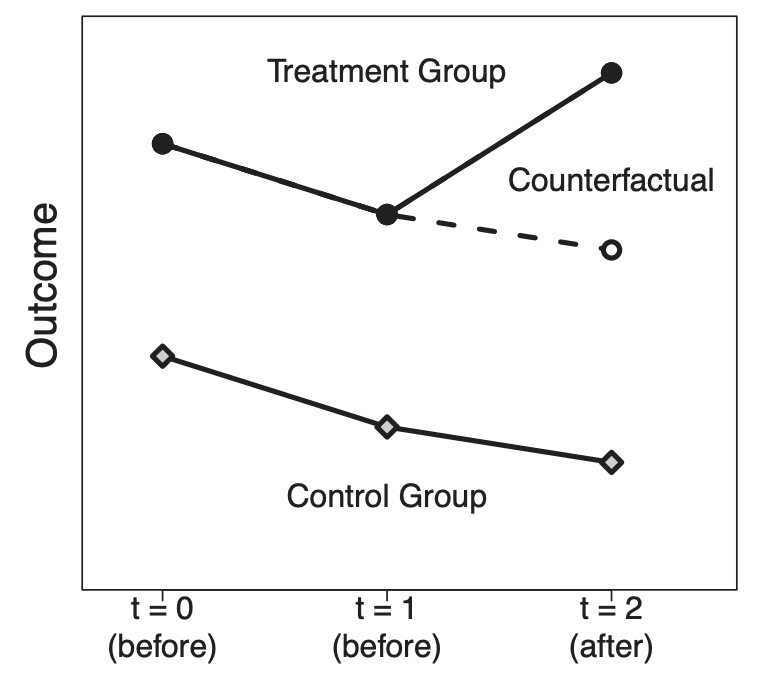
\includegraphics[width = .4\textwidth]{figures/egami_yamauchi_fig2a}}; 
\pause
\node[anchor = north, font = \large] (not) at (ey.south) {Notation};
\draw (not.south west) -- (not.south east);
\node[anchor = north, font = \large] (not2) at (not.south) {$Y_{\text{(unit)(time)}}^{\text{treatment value}}$};
\node[anchor = north, font = \large, align = left] (not3) at (not2.south) {Example: $Y_{i1}^0$\\is unit $i$ at time 1\\under treatment 0};
\pause
\node[anchor = north west, align = left] (pt) at (.5,1) {Parallel Trends Assumption\\(untestable)};
\draw[thick] (pt.south west) -- (pt.south east);
\node[anchor = north west, align = center] at (pt.south west) {$E(Y_{\text{Treated,2}}^0 - Y_{\text{Treated,1}}^0)$\\$=$\\$E(Y_{\text{Control,2}}^0 - Y_{\text{Control,1}}^0)$};
\pause
\node[anchor = north west, align = left] (ept) at (.5,.6) {Extended Parallel Trends\\(testable)};
\draw[thick] (ept.south west) -- (ept.south east);
\node[anchor = north west, align = center] at (ept.south west) {$E(Y_{\text{Treated,1}}^0 - Y_{\text{Treated,0}}^0)$\\$=$\\$E(Y_{\text{Control,1}}^0 - Y_{\text{Control,0}}^0)$};
\end{tikzpicture}

\begin{center}
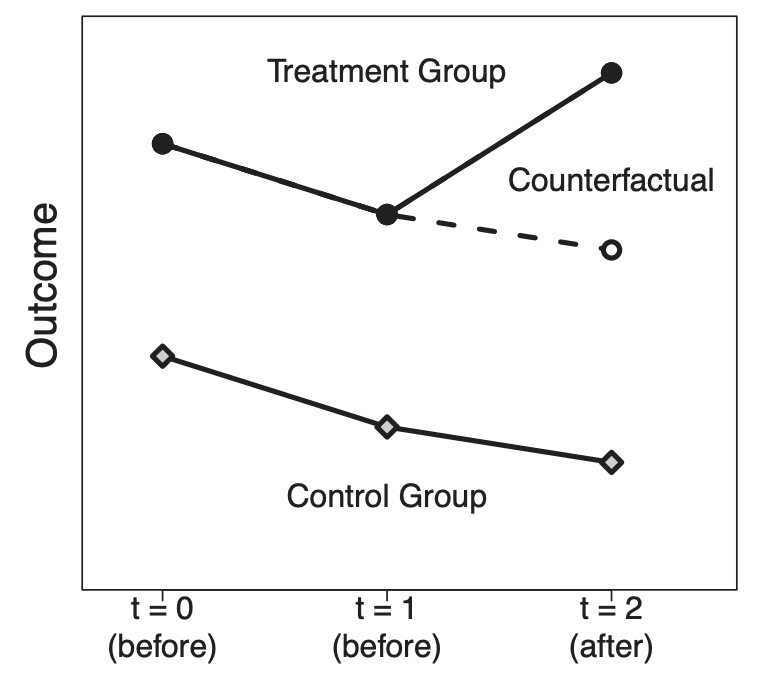
\includegraphics[width = .4\textwidth]{figures/egami_yamauchi_fig2a} \vskip .2in
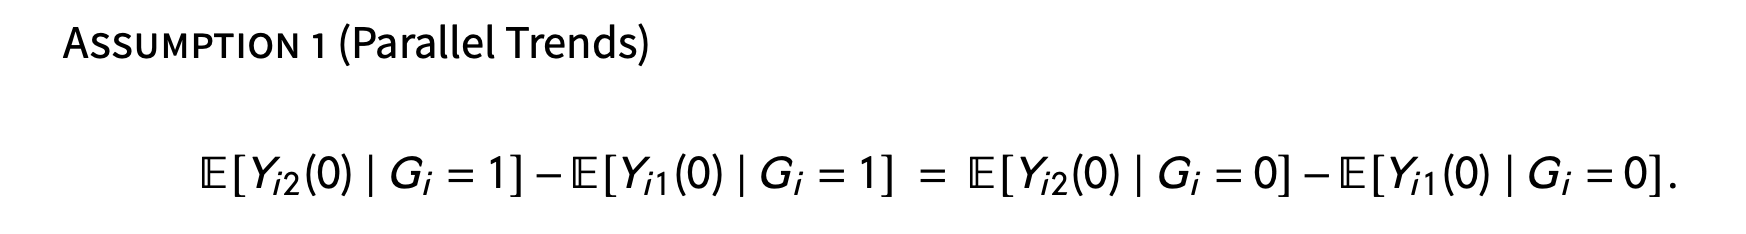
\includegraphics[width = \textwidth]{figures/ey_assumption_1}
\end{center}

\end{frame}

\begin{frame}
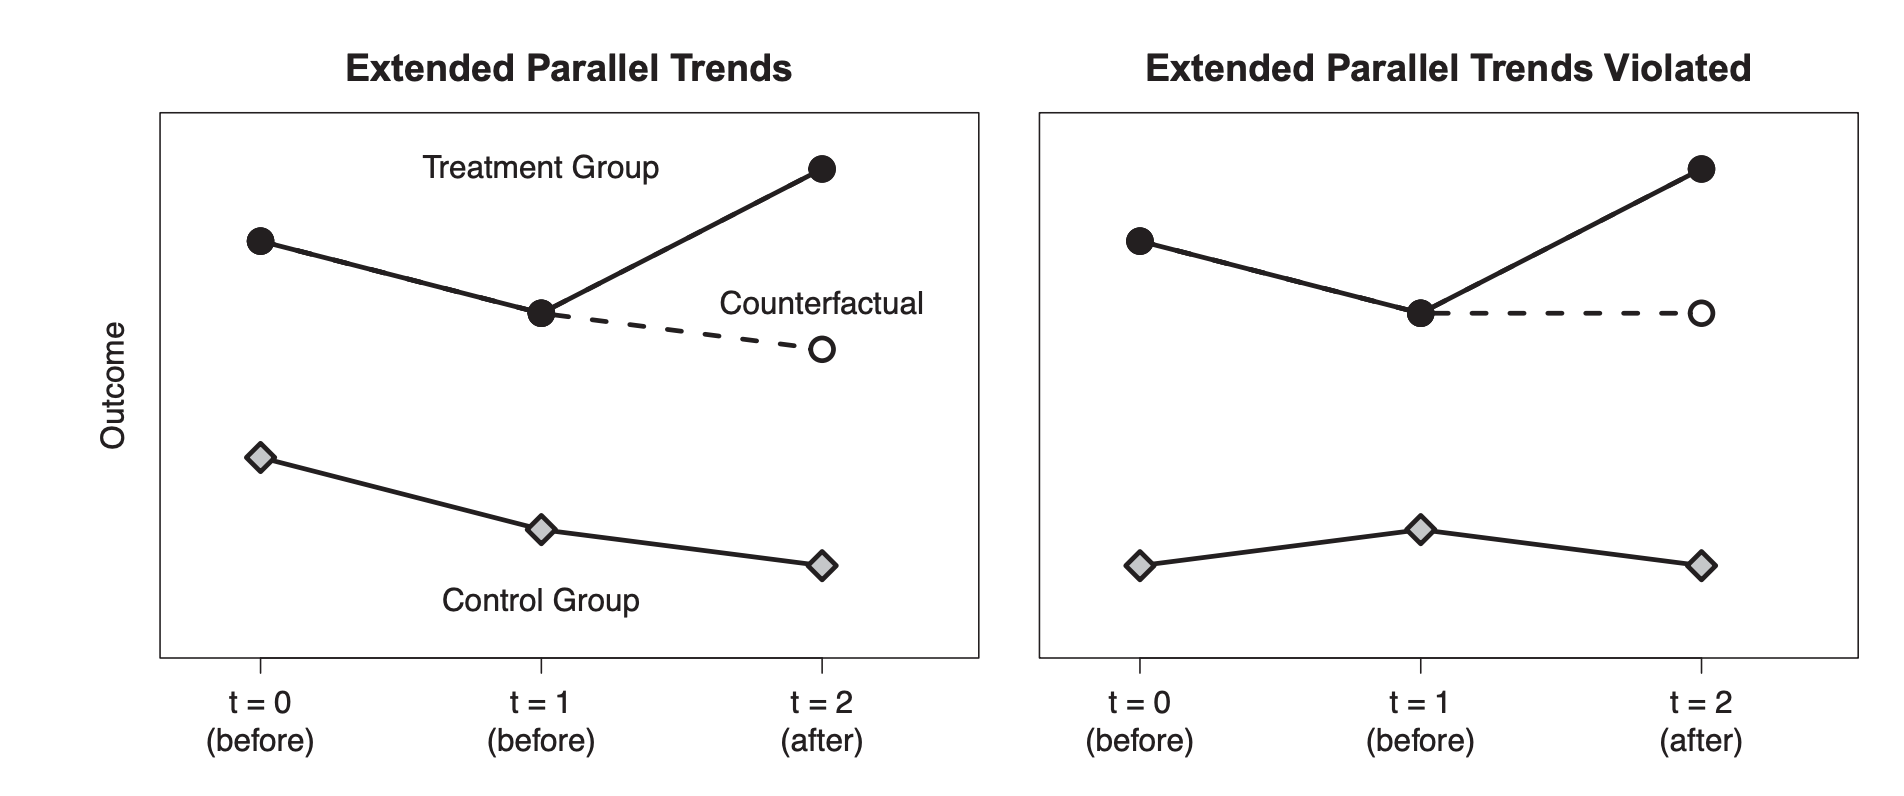
\includegraphics[width = \textwidth]{figures/ey_ept}
\end{frame}

\begin{frame}
\begin{tikzpicture}[x = \textwidth, y = .9\textheight]
\node at (0,0) {};
\node at (1,1) {};
\node[anchor = west] at (0,.5) {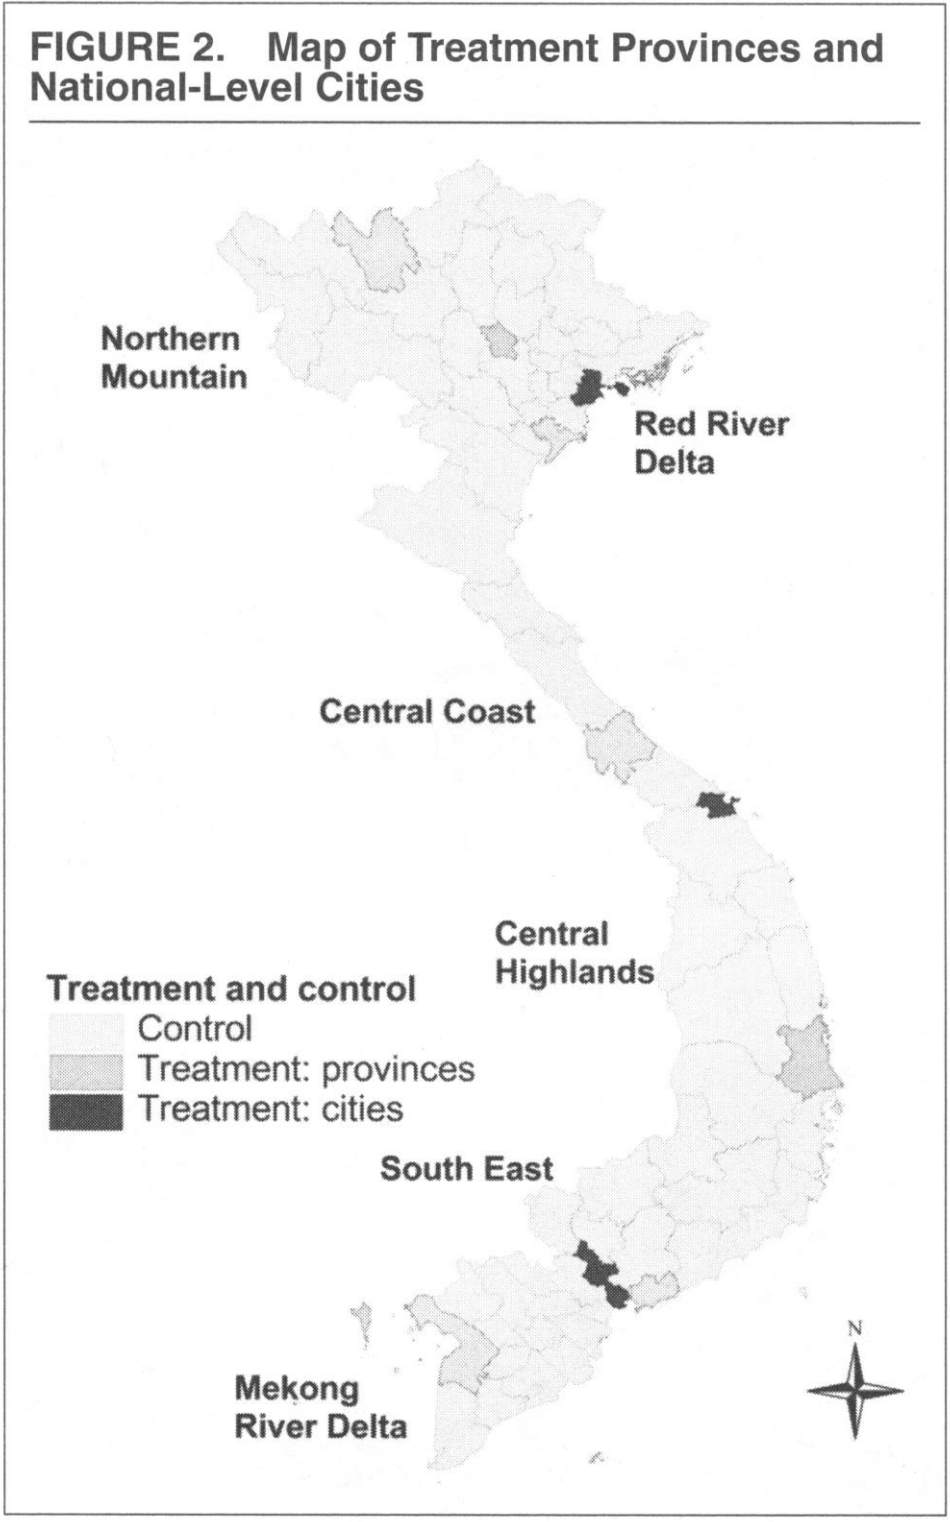
\includegraphics[height = .8\textheight]{figures/malesky_map}};
\onslide<2>{
\node[anchor = north west, align = left] at (.5,1) {Outcome 1\\Education and cultural programs};
\node[anchor = north west, align = left, font = \small, text width = .45\textwidth] at (.5,.85) {\raggedright Is there the following project in the commune?};
\node[anchor = north west, align = left, font = \small, text width = .45\textwidth] at (.55,.73) {\raggedright Investment on culture\\and education};
}
\onslide<3>{
\node[anchor = north west, align = left] at (.5,1) {Outcome 2\\Tap water};
\node[anchor = north west, align = left, font = \small, text width = .45\textwidth] at (.5,.85) {\raggedright Is there the following project in the commune?};
\node[anchor = north west, align = left, font = \small, text width = .45\textwidth] at (.55,.75) {\raggedright \bgray{Coded 1}\\Indoor private piped water\\
Outdoor private piped water\\
Public piped water};
\node[anchor = north west, align = left, font = \small, text width = .45\textwidth] at (.55,.53) {\raggedright \bgray{Coded 0}\\
Well water \\
Well with protection walls \\
Well without protection walls \\
Stream water with protection \\
Stream water without protection \\
Rainwater \\
Bottled water \\
Water brought by pedicab \\
Tank water \\
river lake pond};
}
\onslide<4>{
\node[anchor = north west, align = left] at (.5,1) {Outcome 3\\Agricultural center};
\node[anchor = north west, align = left, font = \small, text width = .45\textwidth] at (.5,.85) {\raggedright Is there any agriculture \\extension center\\in this commune?};
}
\end{tikzpicture}
\end{frame}

\begin{frame}
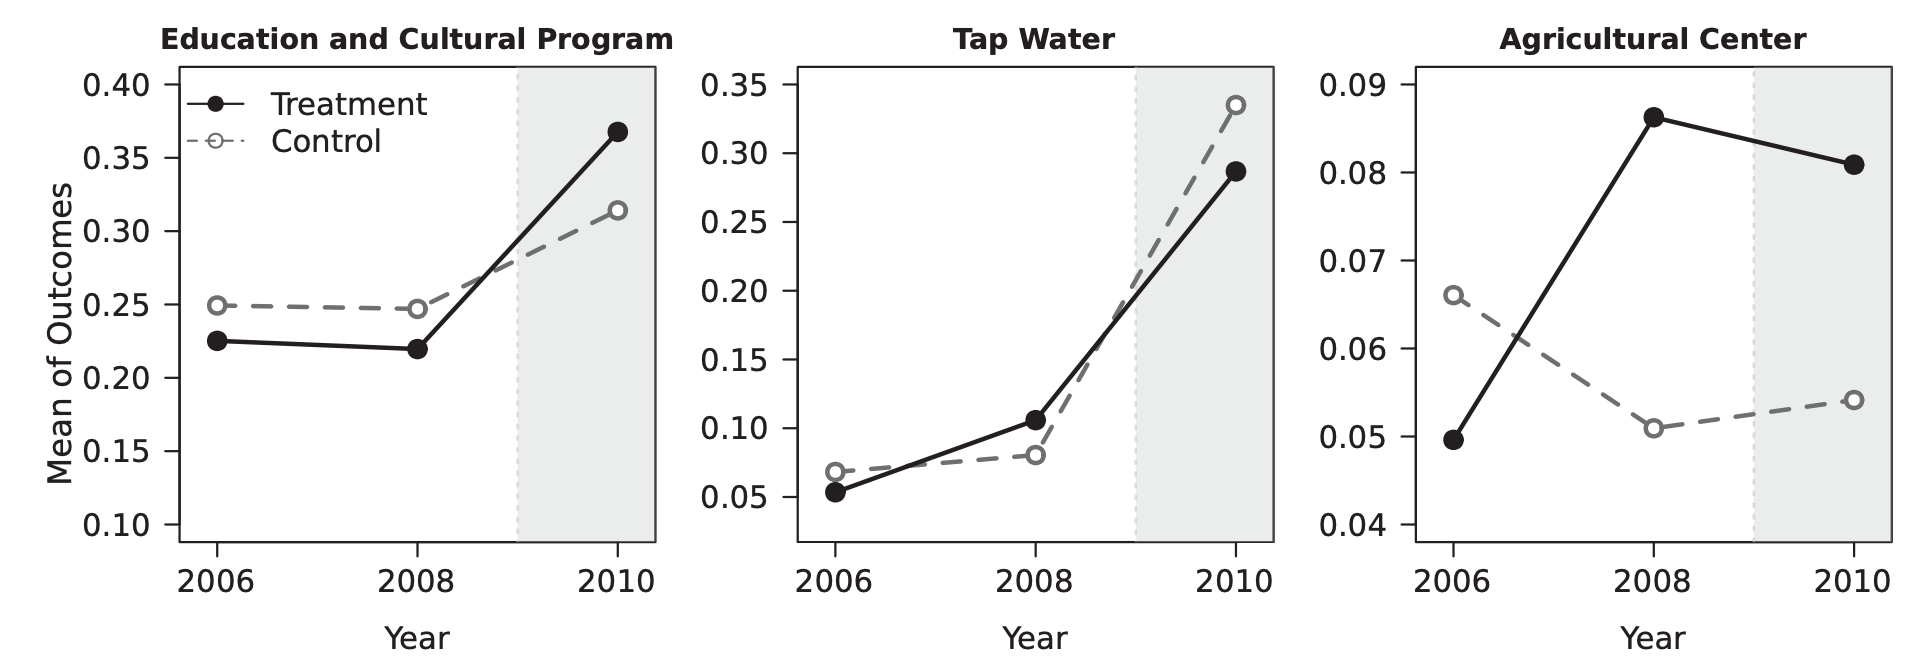
\includegraphics[width = \textwidth]{figures/ey_fig3} \pause \vskip .2in
In each case, do you believe parallel trends? \pause \vskip .2in
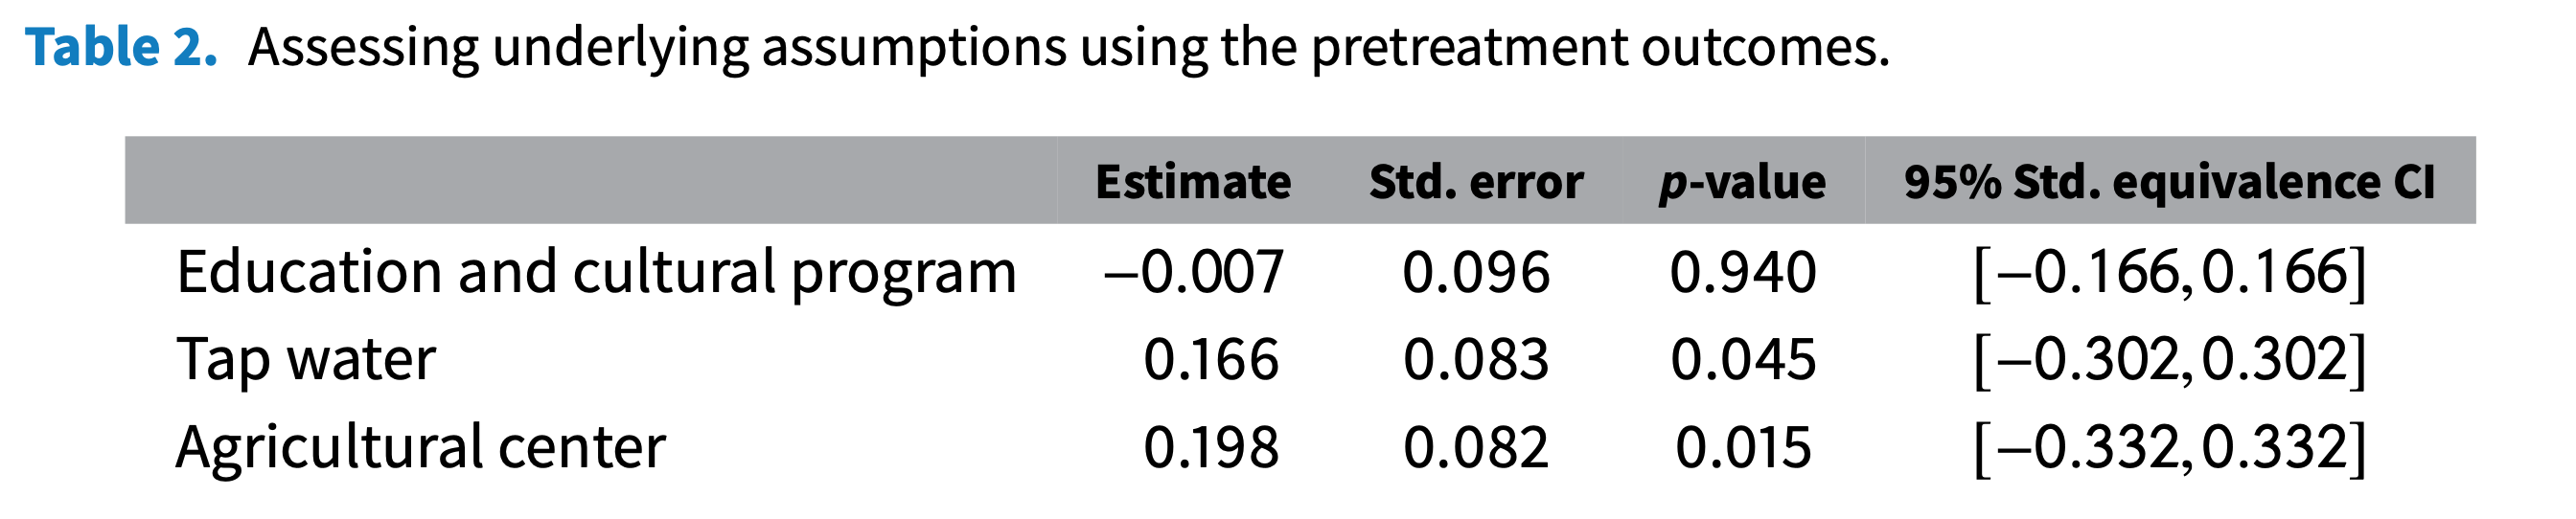
\includegraphics[width = \textwidth]{figures/ey_table2}
\end{frame}

\begin{frame}{Benefit 1: Assessing assumptions}

Pre-treatment periods enable us to\\\bblue{assess underlying ssumptions}\vskip .2in
Parallel trends is untestable, but being parallel \\
in the pre-treatment period builds confidence

\end{frame}

\begin{frame}{Benefit 2: Improving efficiency}

Pre-treatment periods also enable us to\\\bblue{improve estimation accuracy}\\when parallel trends holds

\end{frame}

\begin{frame}{Benefit 2: Improving efficiency}
\begin{tikzpicture}[x = \textwidth, y = .9\textheight]
\node at (0,0) {};
\node at (1,1) {};
\node[anchor = north west] (ey) at (0,1) {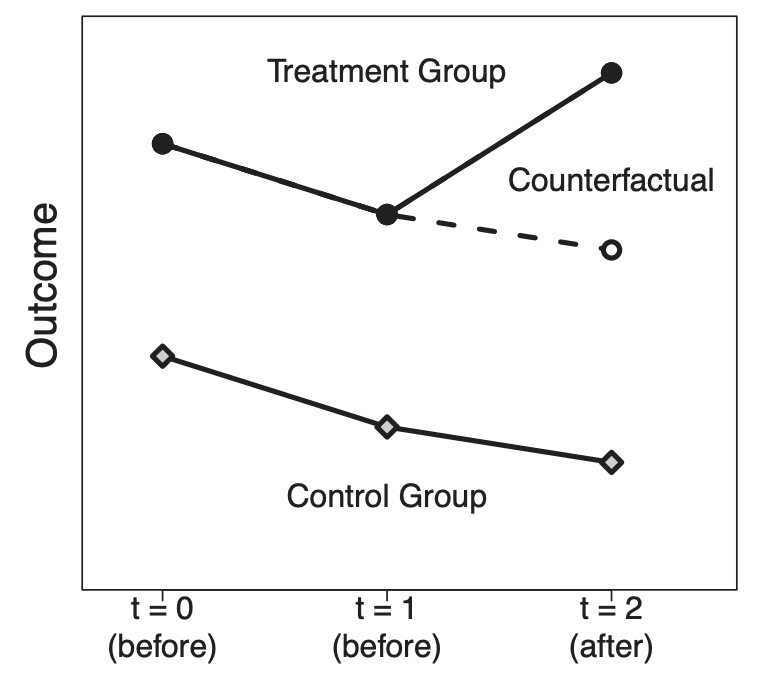
\includegraphics[width = .4\textwidth]{figures/egami_yamauchi_fig2a}}; 
\node[anchor = north, font = \large] (not) at (.25,.4) {Notation};
\draw (not.south west) -- (not.south east);
\node[anchor = north, font = \large] (not2) at (not.south) {$Y_{\text{(unit)(time)}}^{\text{treatment value}}$};
\node[anchor = north west] (est1) at (.5,1) {Estimator 1};
\node[anchor = north west] (est2) at (.5,.7) {Estimator 2};
\pause
\node[anchor = north west, align = center] at (est1.south west) {$\underbrace{(\bar{Y}_{T2}^1 - \bar{Y}_{T1}^0)}_{\substack{\text{Treatment Group}\\\text{Time 2 - Time 1}}}-\underbrace{(\bar{Y}_{C2}^0 - \bar{Y}_{C1}^0)}_{\substack{\text{Control Group}\\\text{Time 2 - Time 1}}}$};
\pause
\node[anchor = north west, align = center] at (est2.south west) {$\underbrace{(\bar{Y}_{T2}^1 - \bar{Y}_{T0}^0)}_{\substack{\text{Treatment Group}\\\text{Time 2 - Time 0}}}-\underbrace{(\bar{Y}_{C2}^0 - \bar{Y}_{C0}^0)}_{\substack{\text{Control Group}\\\text{Time 2 - Time 0}}}$};
\pause
\node[anchor = north west, font = \bf, blue, align = left] at (.5,.35) {Pooled estimator:\\Average the two!};
\end{tikzpicture}

\end{frame}

\begin{frame}{Benefit 2: Improving efficiency}
\centering
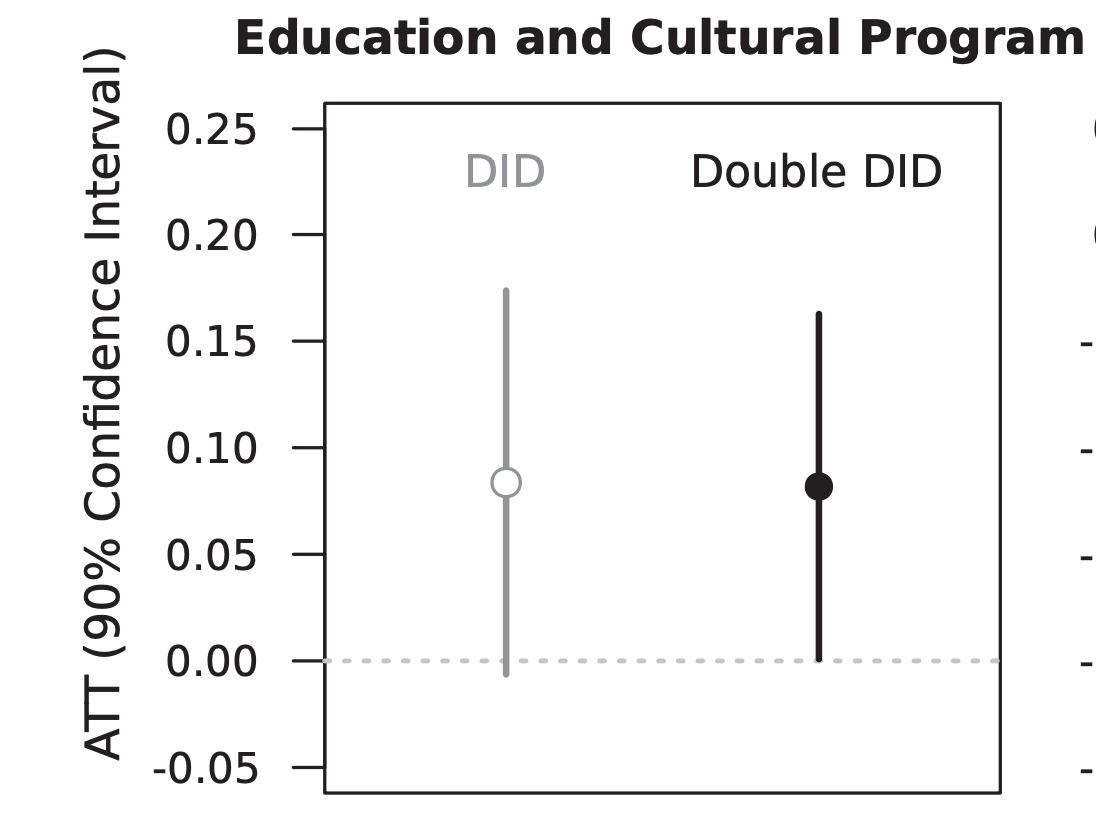
\includegraphics[width = .5\textwidth]{figures/ey_fig4a}
\end{frame}

\begin{frame}{Benefit 3: A more flexible assumption}

Pre-treatment periods make it possible to\\
\bblue{allow for a more flexible parallel trends assumption}

\end{frame}

\begin{frame}{Benefit 3: A more flexible assumption}
\begin{tikzpicture}[x = \textwidth, y = .9\textheight]
\node at (0,0) {};
\node at (1,1) {};
\node[anchor = west] at (0,.5) {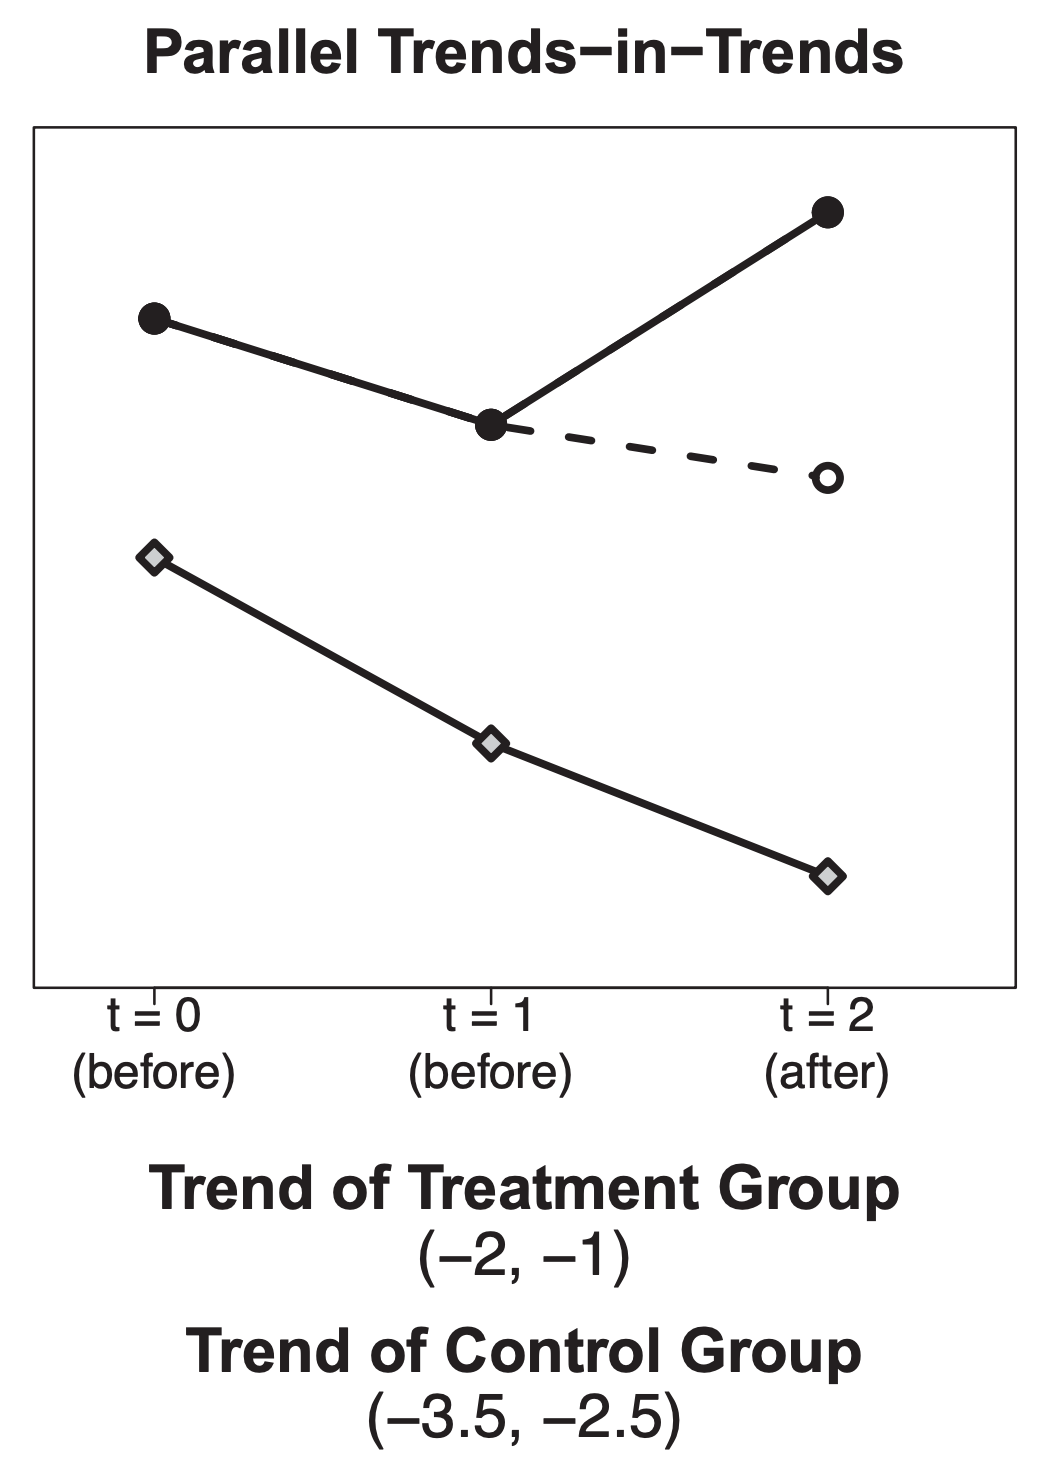
\includegraphics[height = .5\textheight]{figures/ey_fig2b}}; \pause
\node[anchor = north east] at (1,.8) {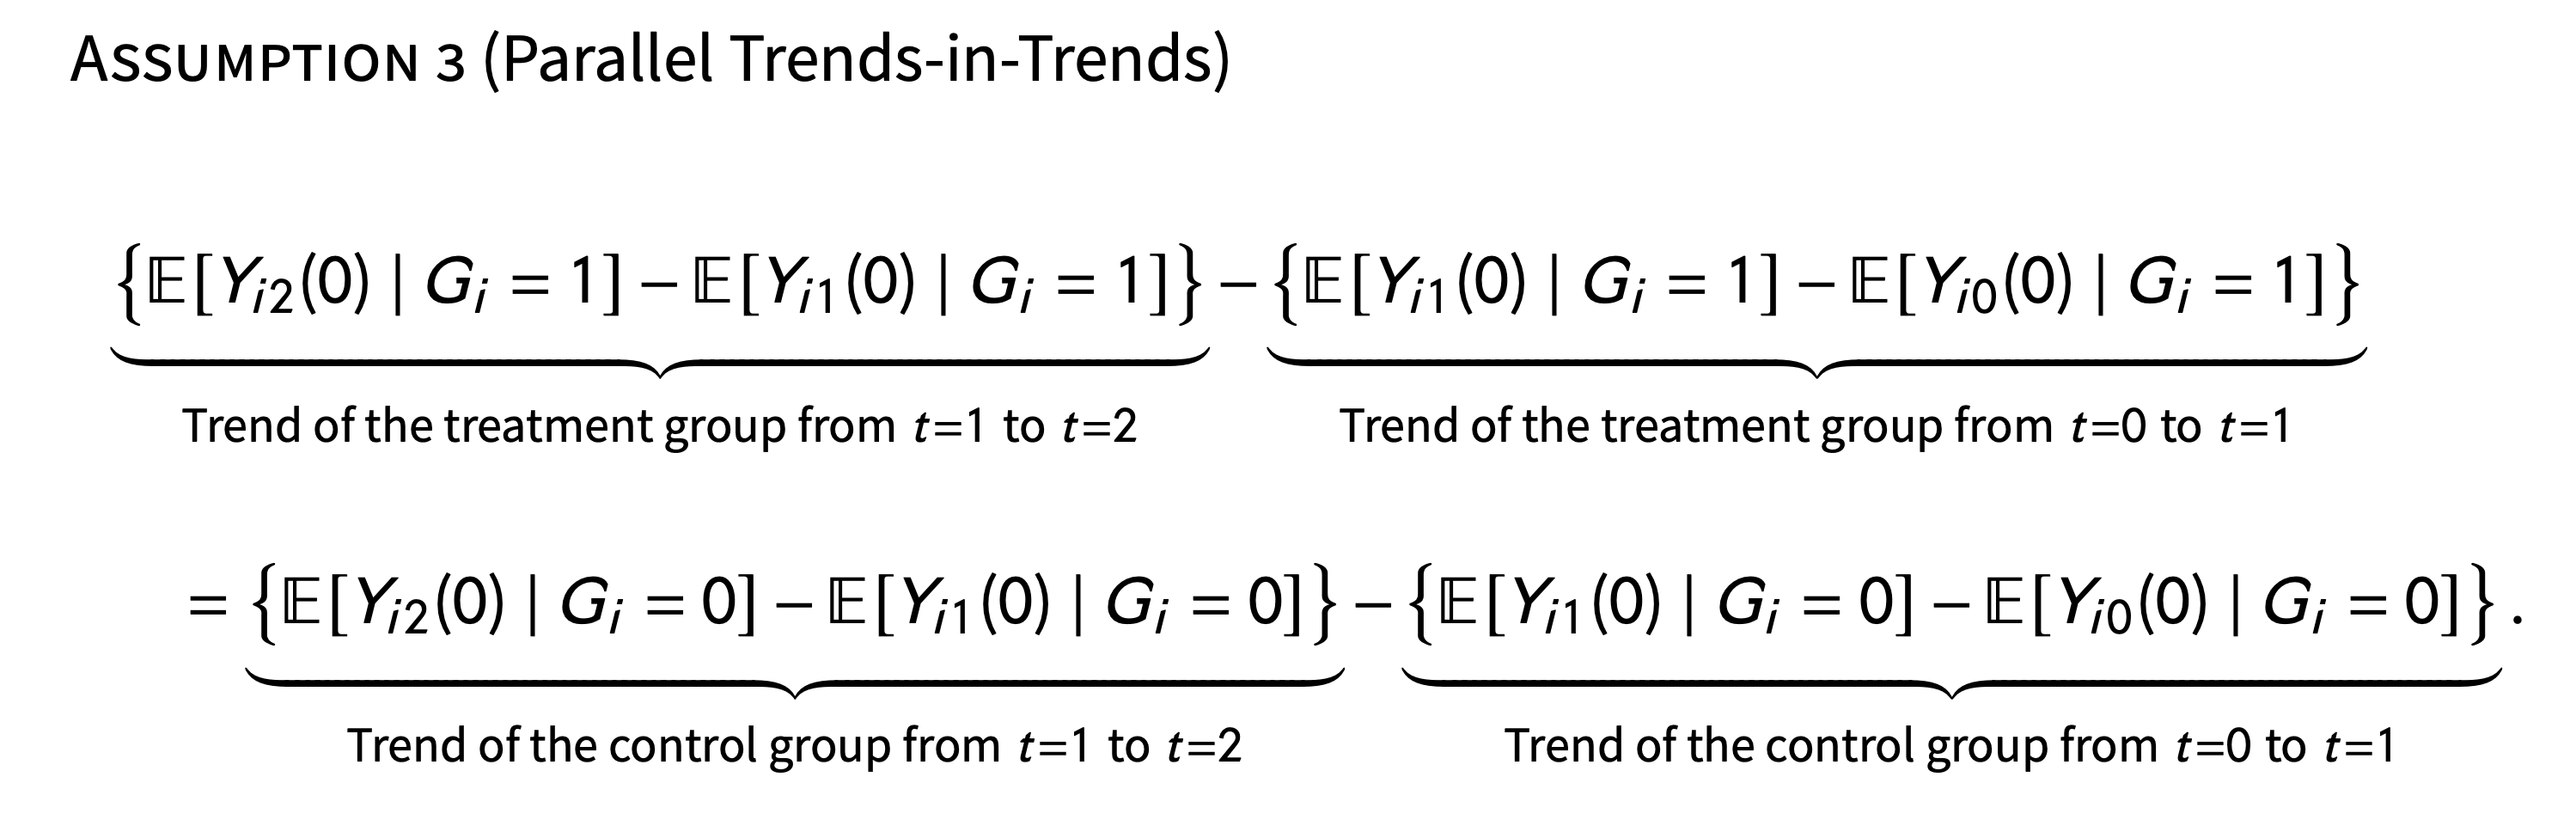
\includegraphics[width = .65\textwidth]{figures/ey_assumption3}}; \pause
\node[anchor = north west] at (.35,.47) {Sequential DID Estimator};
\node[anchor = north west] at (.35,.4) {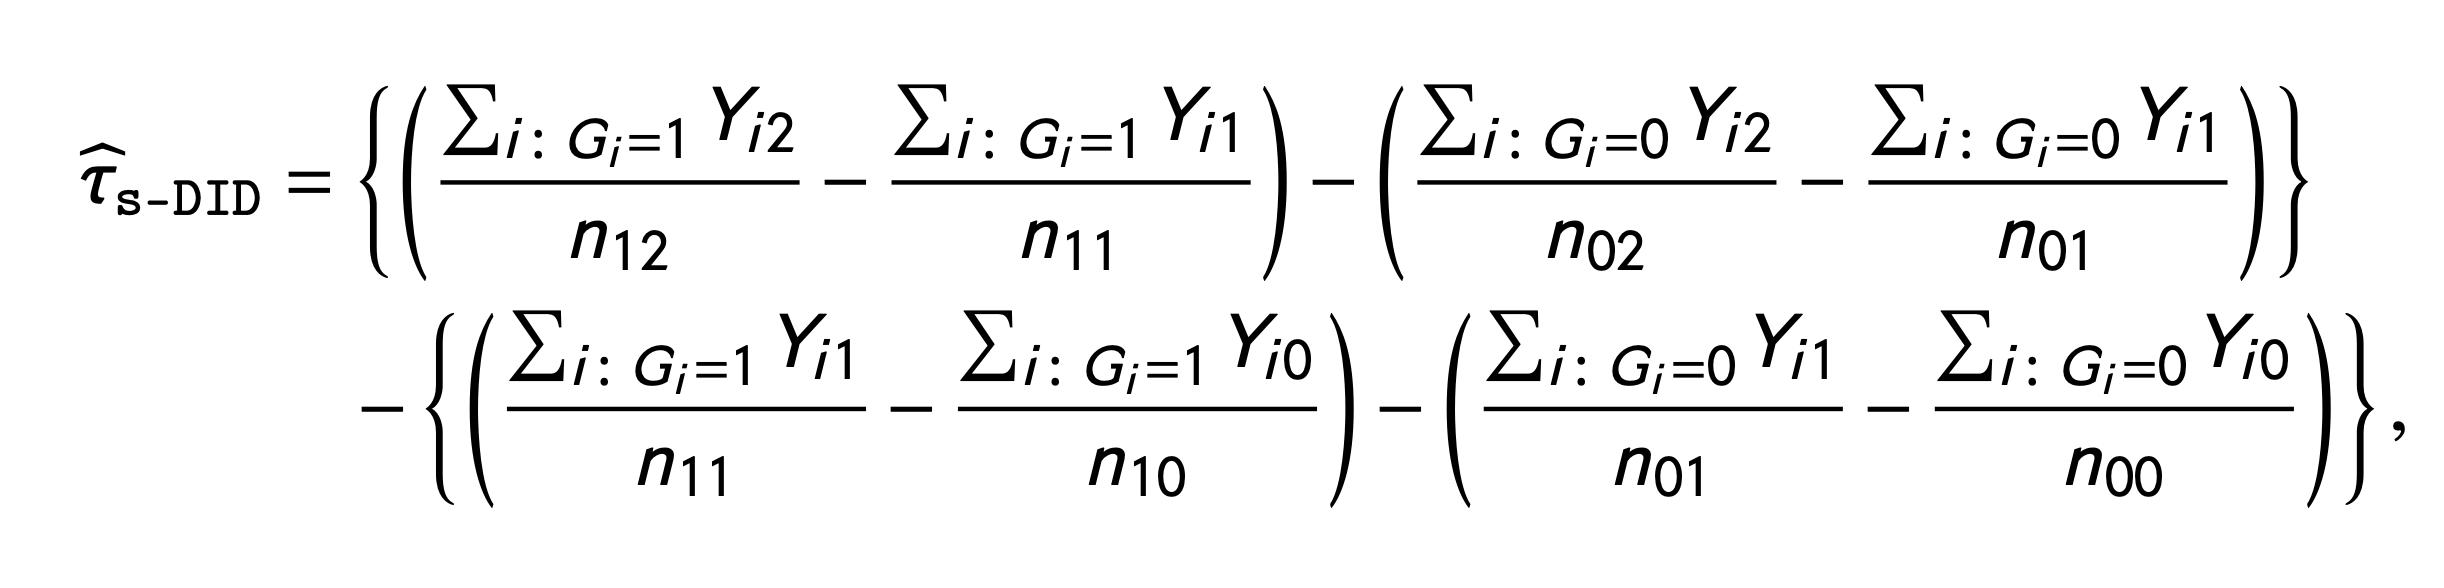
\includegraphics[width = .65\textwidth]{figures/ey_sdid}};
\end{tikzpicture}
\end{frame}

\begin{frame}{Benefit 3: A more flexible assumption}
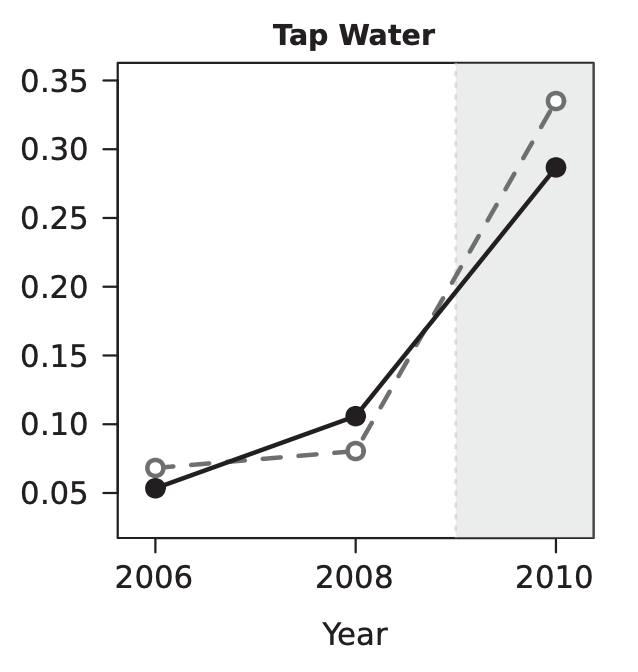
\includegraphics[width = .4\textwidth]{figures/ey_fig3b} \qquad
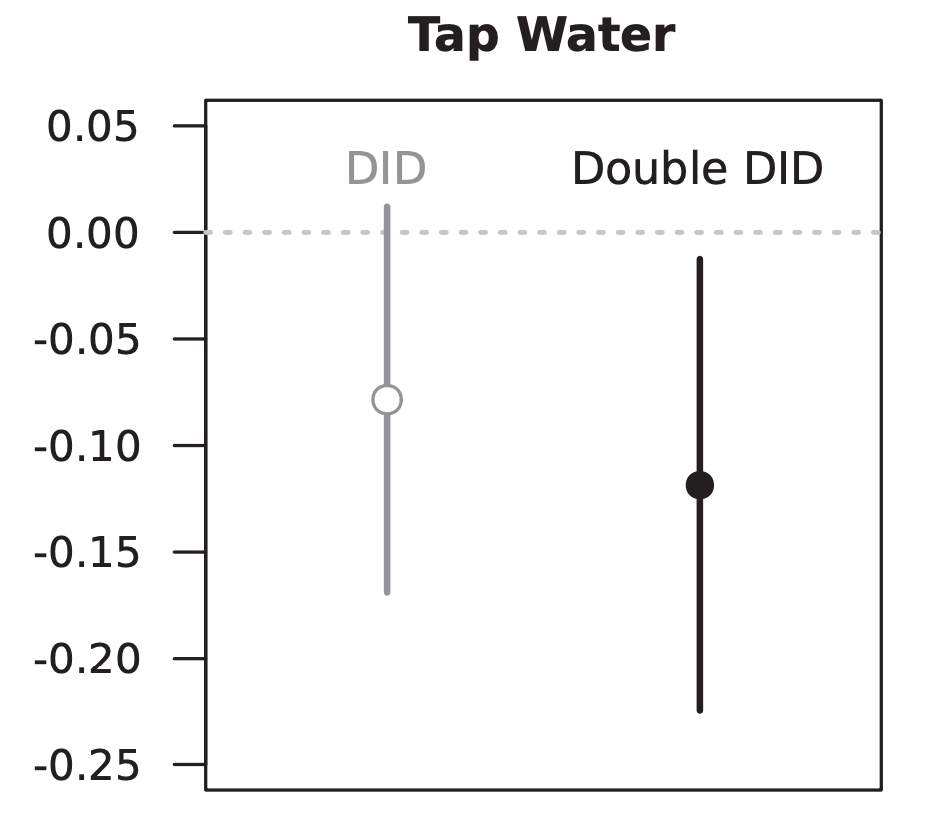
\includegraphics[width = .4\textwidth]{figures/ey_fig4b}
\end{frame}

\begin{frame}{Benefits of multiple pre-treatment periods}

\begin{enumerate}
\item assess underlying assumptions
\item improve estimation accuracy
\item allow for a more flexible parallel trends assumption
\end{enumerate}
\begin{tikzpicture}[x = \textwidth, y = .6\textheight]
\node at (0,0) {};
\node at (1,1) {};
\node<2> at (.5,.5) {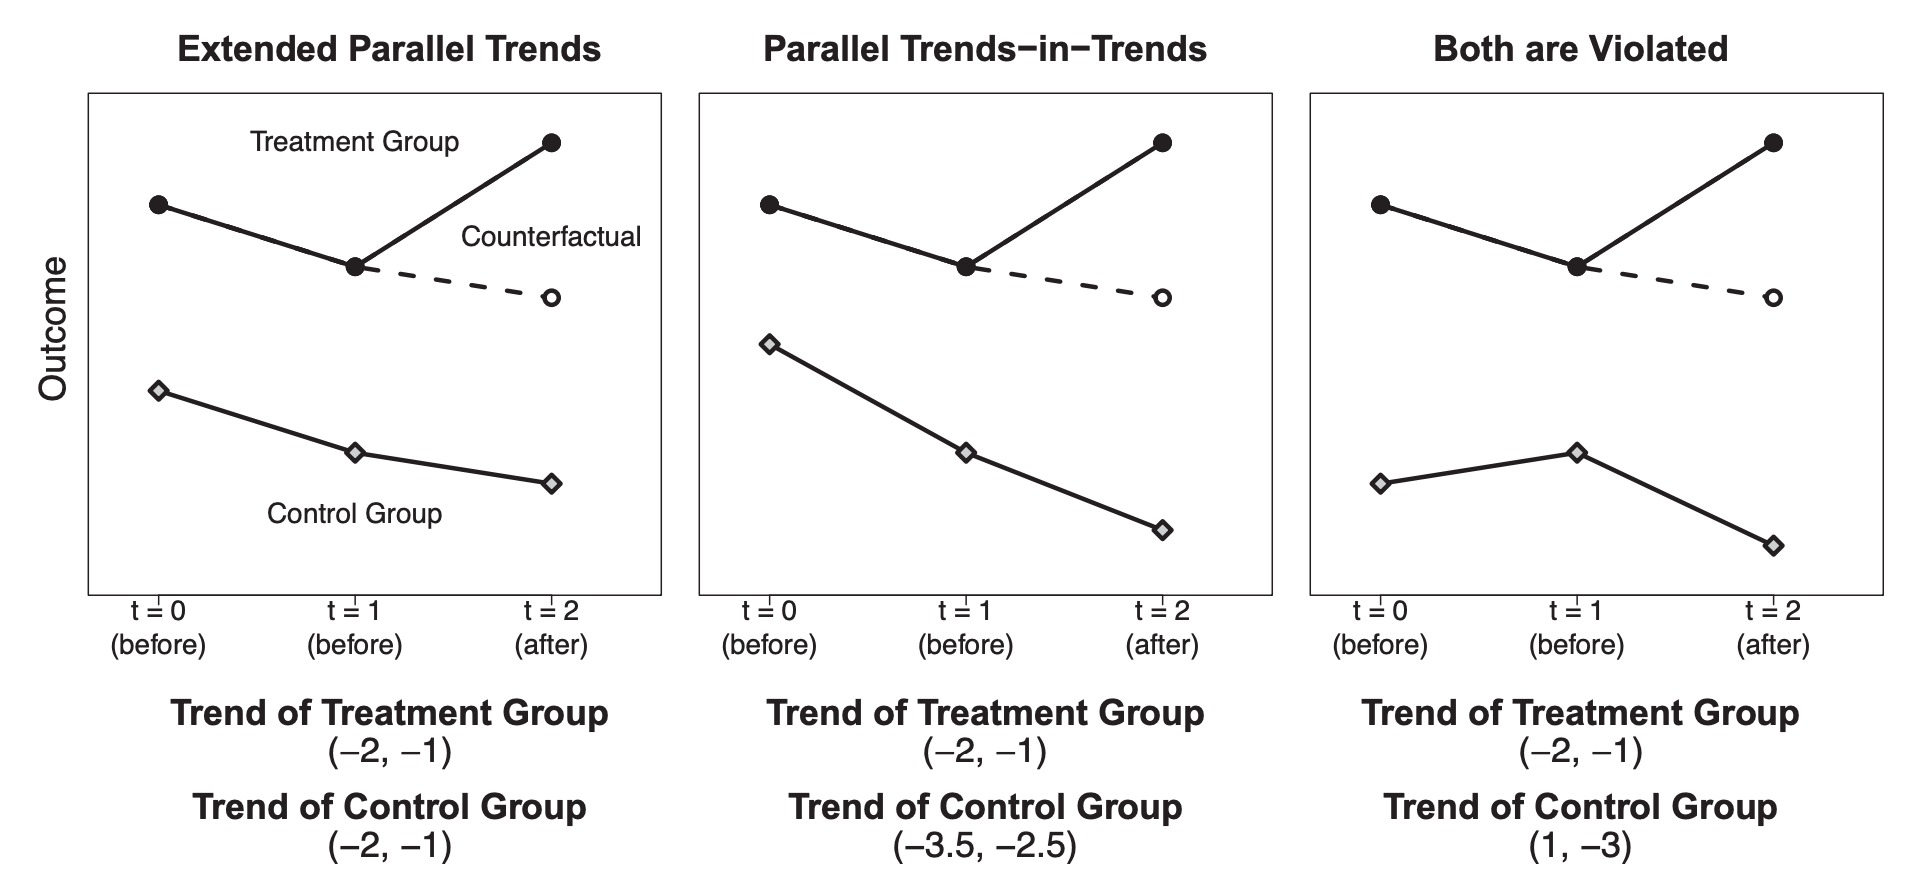
\includegraphics[width = \textwidth]{figures/ey_fig2}};
\node<3> at (.5,.5) {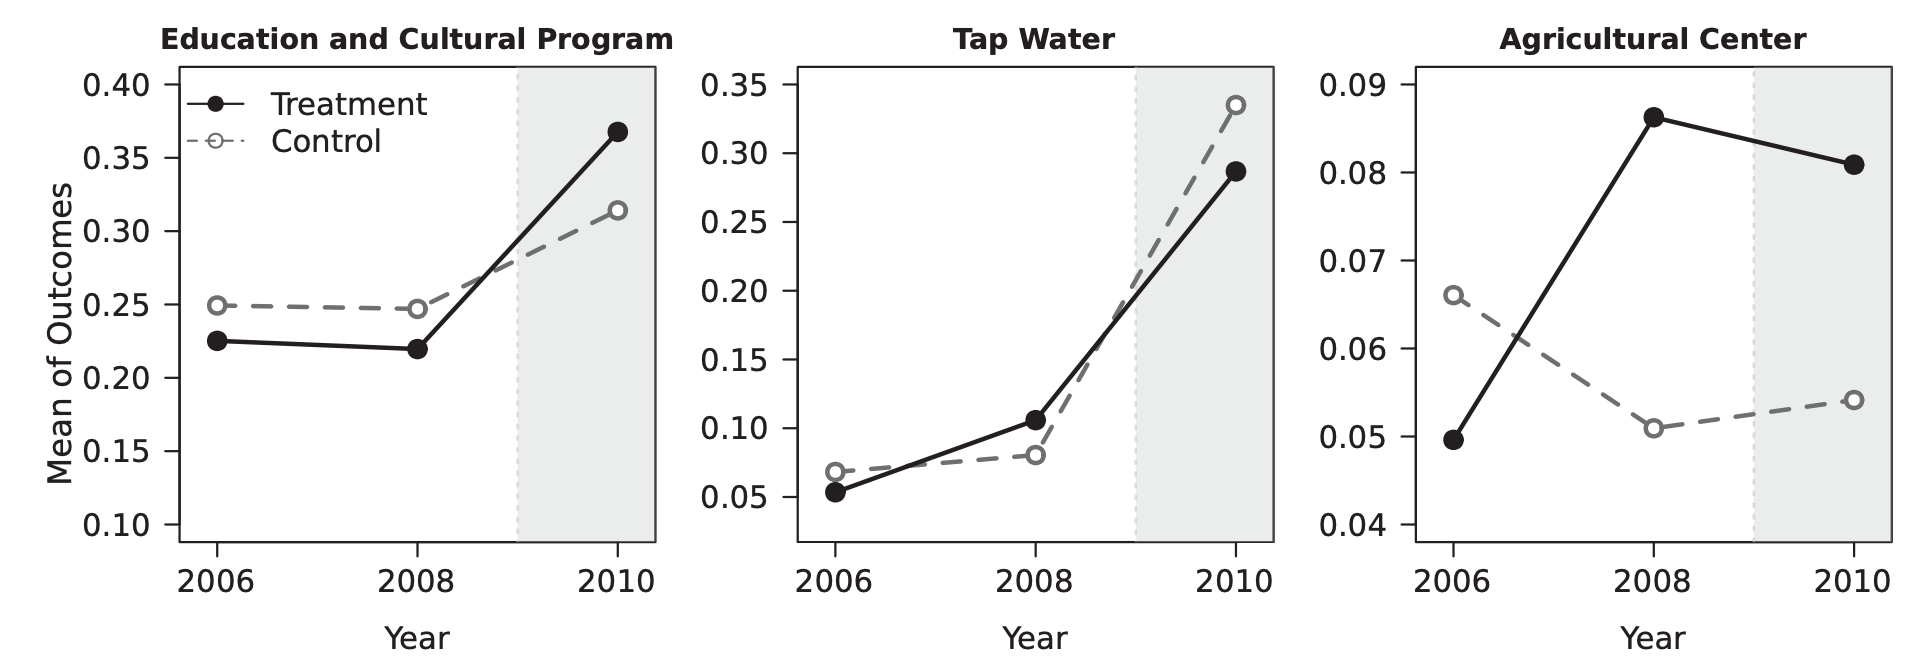
\includegraphics[width = \textwidth]{figures/ey_fig3}};
\end{tikzpicture}
\end{frame}

\goalsframe


\end{document}
